%%%%%%
% $Beschreibung: Poster des Demonstrators mit erklärung eines Schrittmotors $
% $Autor: Groenke $
% $Datum: 18.06.2024 $
% $Version: 1 $
% $Pfad: SchrittmotorArduino/Poster/tikzposter.tex $
%
%%%%%%

\documentclass[25pt,a0paper, portrait]{tikzposter}
\usepackage[utf8]{inputenc}
\usepackage{xcolor}
\usepackage{graphicx,mwe}
\usepackage{filecontents}
\usepackage{lipsum}
\usepackage{tikz}
\usepackage{multicol}
\usepackage{adjustbox}
\usepackage{blindtext}
\usepackage{comment}


 \makeatletter
\def\TP@titlegraphictotitledistance{-6cm}
\settitle{ \centering \vbox{
		\@titlegraphic \\ [\TP@titlegraphictotitledistance] 
		\centering
		\color{titlefgcolor} 
		{\bfseries \Huge \sc \@title \par}
		\vspace*{1em}
		{\huge \@author \par}
}}
\makeatother

\setlength{\columnsep}{2cm}
 
\title{Schrittmotor Demonstrator}
\author{A24-27}
\titlegraphic{
\includegraphics[height=6.5cm]{images/logo_hs_technik}
	\hfill

\includegraphics[height=6.5cm]{images/logo}
}
 
 
\usetheme{Desert}
 
\begin{document}

 
\maketitle

\begin{columns} 
	
	\column{0.4}
	{
		\colorlet{blocktitlebgcolor}{blue}
		\block{Demonstrator für einen Schrittmotor}
		{
			\begin{tikzfigure}
				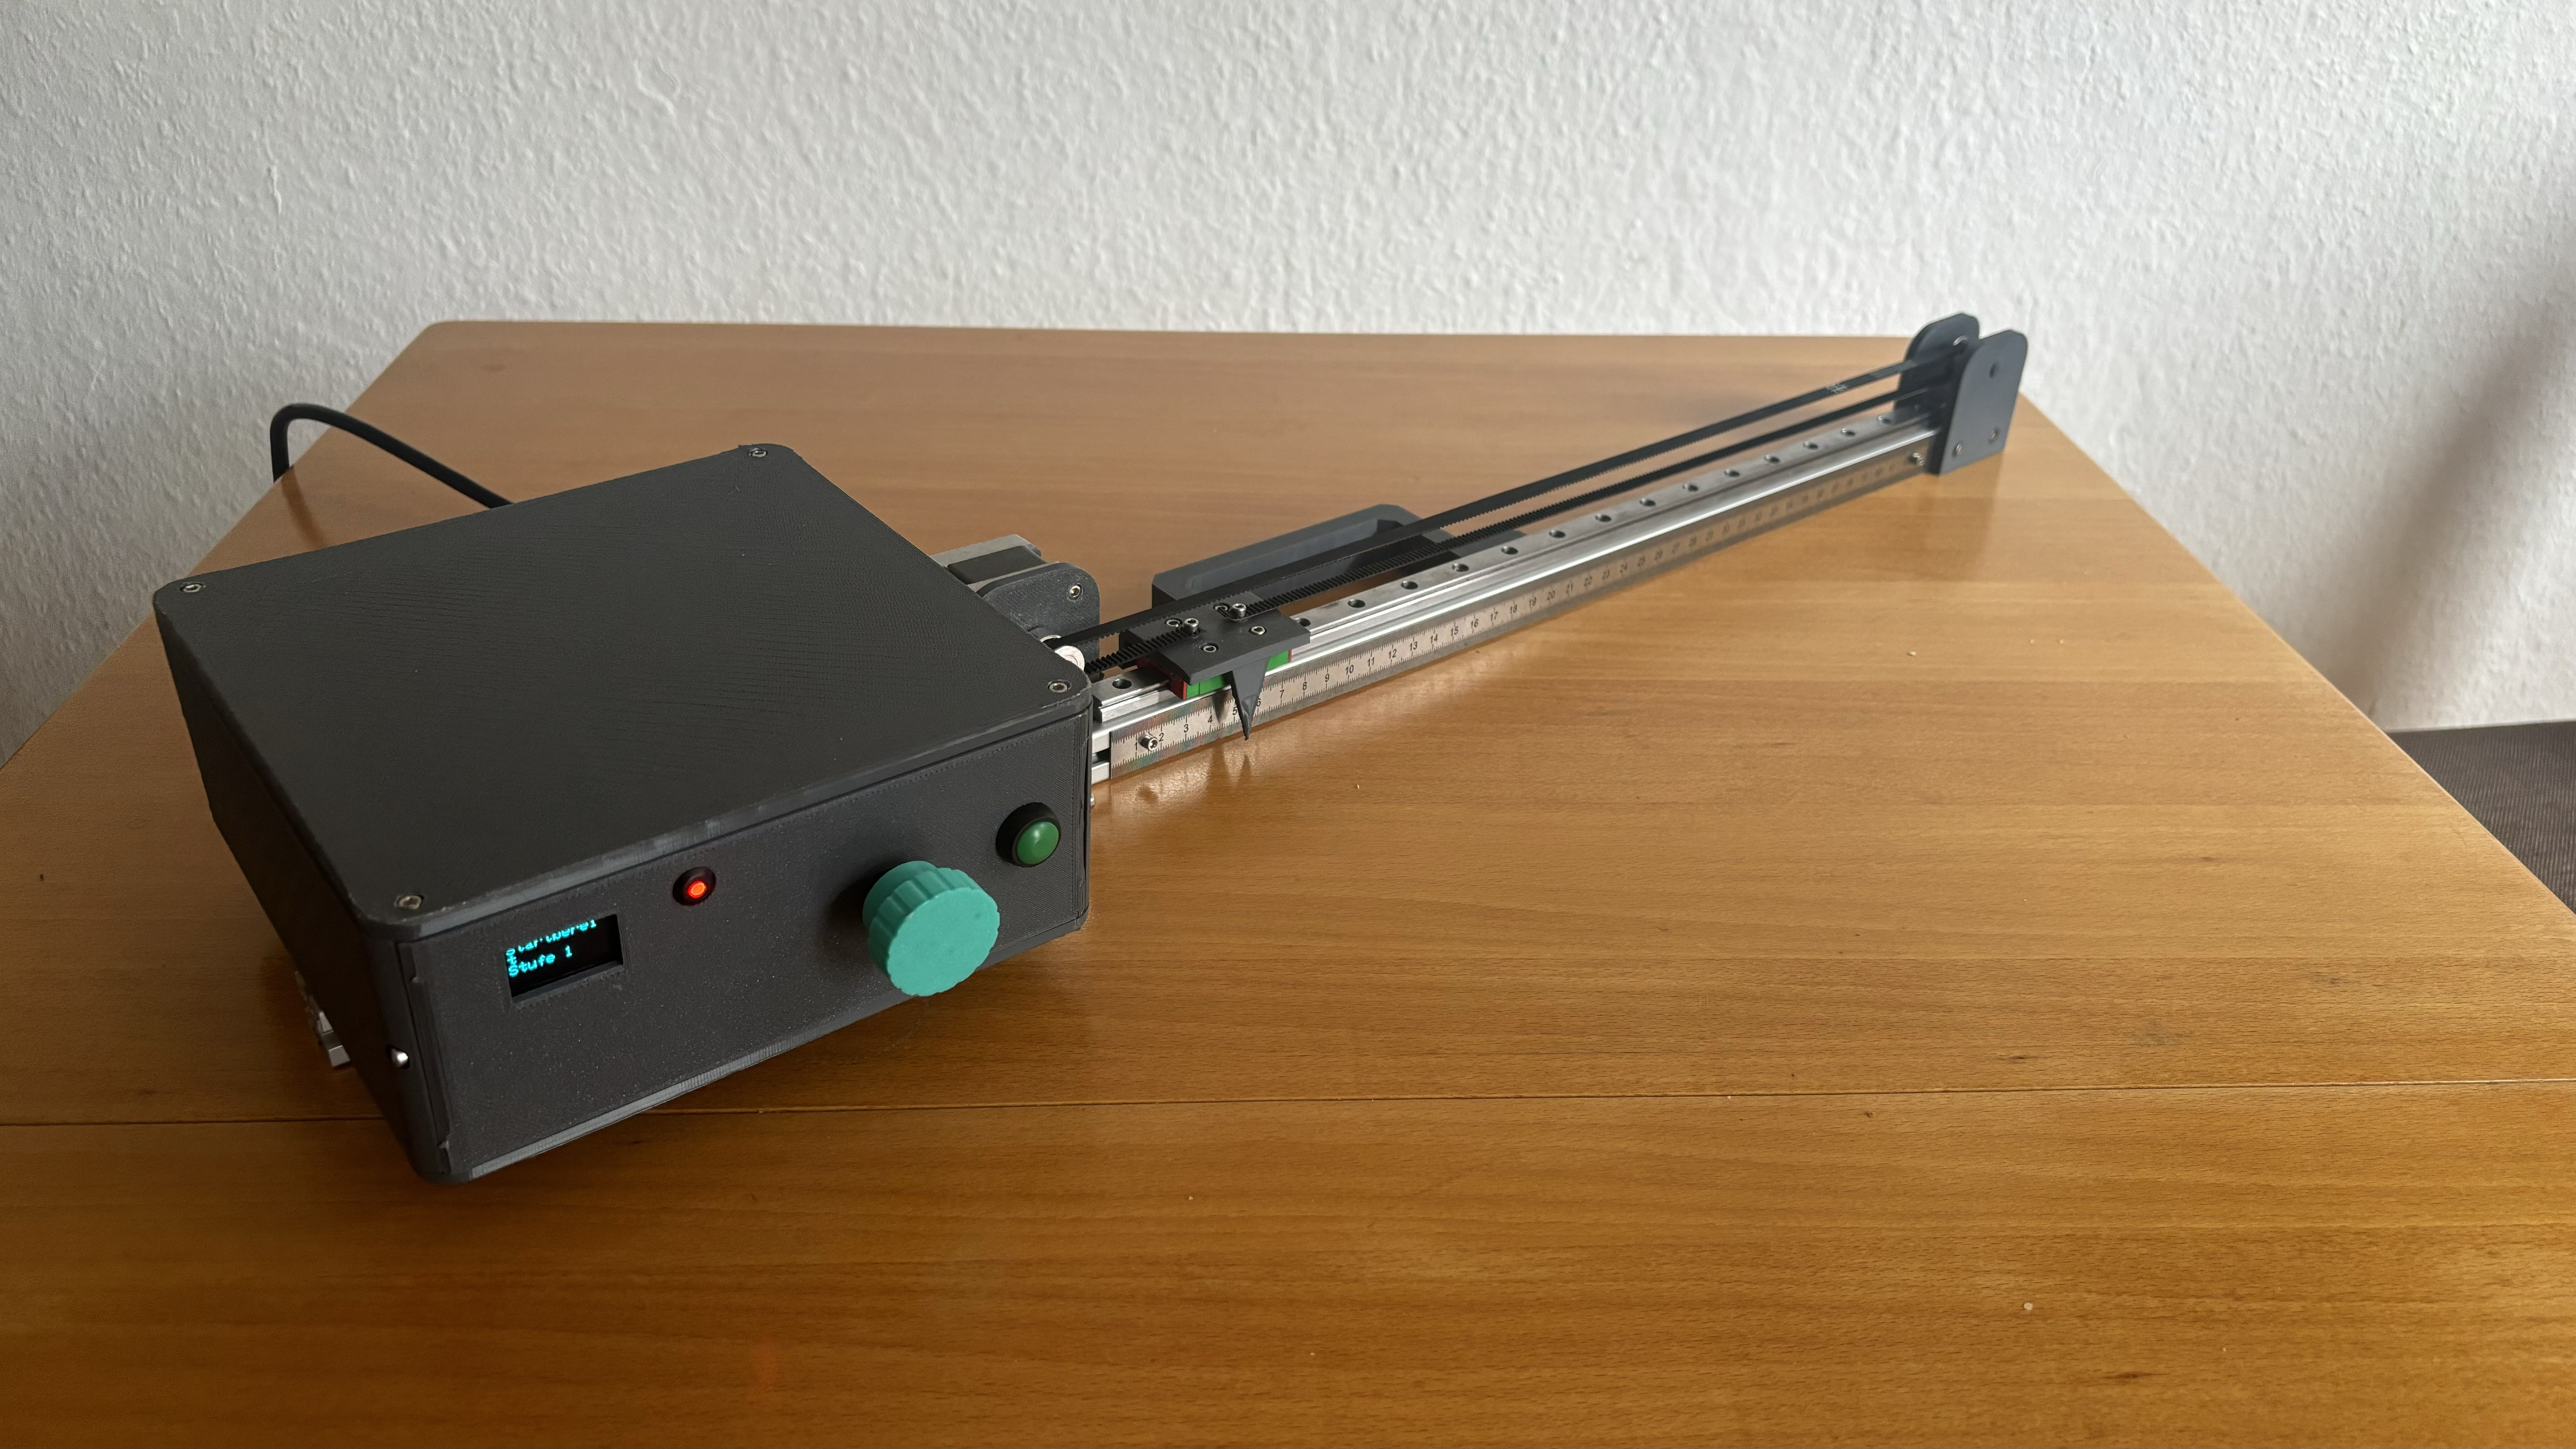
\includegraphics[width=\linewidth]{images/DemonstratorDrauf}
			\end{tikzfigure}	
		}
		\block{Schrittmotoren}
		{
			Ein Schrittmotor ist ein Elektromotor, der sich für präzise Positionierungsaufgaben eignet. Im Gegenteil zu anderen Elektromotoren wird bei einem Schrittmotor keine Positionsmessung oder Positionsregelung benötigt. Mit	diesem Motor ist eine erreichbare Positioniergenauigkeit von 0,1° möglich. Diese Art von Elektromotor wird beispielsweise in Druckern oder Scanner, aber auch im Kraftfahrzeugbereich verwendet. Im Kraftfahrzeugbereich werden die Schrittmotoren zur Spiegelverstellung sowie der Sitzverstellung verwendet. Das maximal erreichbare Drehmoment eines Schrittmotors liegt bei zwei Newtonmeter und die maximal erreichbare Drehzahl bei ca. 2000 Umdrehung pro Minute. Ein großer Vorteil des Schrittmotors ist seine Wartungsfreiheit, da der Rotor keine Wicklungen hat. [Babiel 2023, Hagl 2021]
		}
	}


	\column{0.6}
	{
		\colorlet{blocktitlebgcolor}{blue}
		\block{Projektbeschreibung}
		{
			Mithilfe eines Arduino Nano 33 BLE Sense Lite wurde dieser Demonstrator für einen Schrittmotor entwickelt. Mittels einer Konstruktion, die über einen Schrittmotor verfügt, wird ein Riemen angetrieben. An diesem Riemen ist ein Schlitten befestigt, der durch die Bewegung des Schrittmotors auf einer Linearerführung verfahren wird. An dem Gehäuse befindet sich ein Drehschalter, mit dem eine von zehn Bewegungsstufen ausgewählt werden kann. Nach der Auswahl kann das Programm über den grünen Start-Stopp-Knopf gestartet werden. Die Status-LED leuchtet rot, sobald das Gerät einsatzbereit ist. Für die Referenzfahrt wurde ein Endschalter an der Halterung des Schrittmotors befestigt, damit der Schrittmotor auf eine definierte Position referenzieren kann. Es gibt zehn verschiedene Bewegungsstufen. Die Bewegungsstufen unterscheiden sich in der Geschwindigkeit. Pro Stufe wird die Geschwindigkeit erhöht.
			Ein großer Teil der Bauteile wurde mit einem 3D-Drucker gefertigt. So konnten Gehäuse, Drehschalter, Zeiger (auf dem Schlitten), Halterungen, sowie ein Griff selbst konstruiert und angepasst werden. 
		}
		\block{Nema 17 Schrittmotor}
		{
			Für dieses Projekt wird ein Nema 17 Schrittmotor der Firma Creality3D verwendet. Dieser Schrittmotor wird im 3D-Druck sowie in CNC-Maschinen eingesetzt. Der Motor arbeitet im Bipolarbetrieb und es sind zwei Spulen verbaut. Er hat einen Schrittwinkel von 1,8 ° und
			benötigt somit 200 Schritte für eine volle Umdrehung. Die Wellenlänge beträgt 20 mm und der Wellendurchmesser 5 mm. Der ausgewählte Schrittmotor arbeitet mit einer Nennspannung von 12 Volt. Dadurch, dass er mit einer niedrigen Spannung arbeitet, kann kein hohes Drehmoment erzeugt werden. Allerdings erzielt der Schrittmotor eine gute Positioniergenauigkeit durch den kleinen Schrittwinkel und das Microstepp-Funktion. Des Weiteren arbeitet der Motor mit 0,84 Amper pro Phase. Weitere Vorteile des Schrittmotors sind die kompakte Bauform mit den Abmessung 42 x 42 x 34 mm sowie die geringe Masse von 220 Gramm. Betrieben werden kann der Schrittmotor in einer Umgebungstemperatur von -20 °C bis +50 °C. [Gemsmotor 2024] 
		}
	}
\end{columns}

\begin{columns} 
	
	\column{0.4}
	{
		\colorlet{blocktitlebgcolor}{blue}
		\block{Nema 17 Schrittmotor}
		{
			\begin{tikzfigure}
				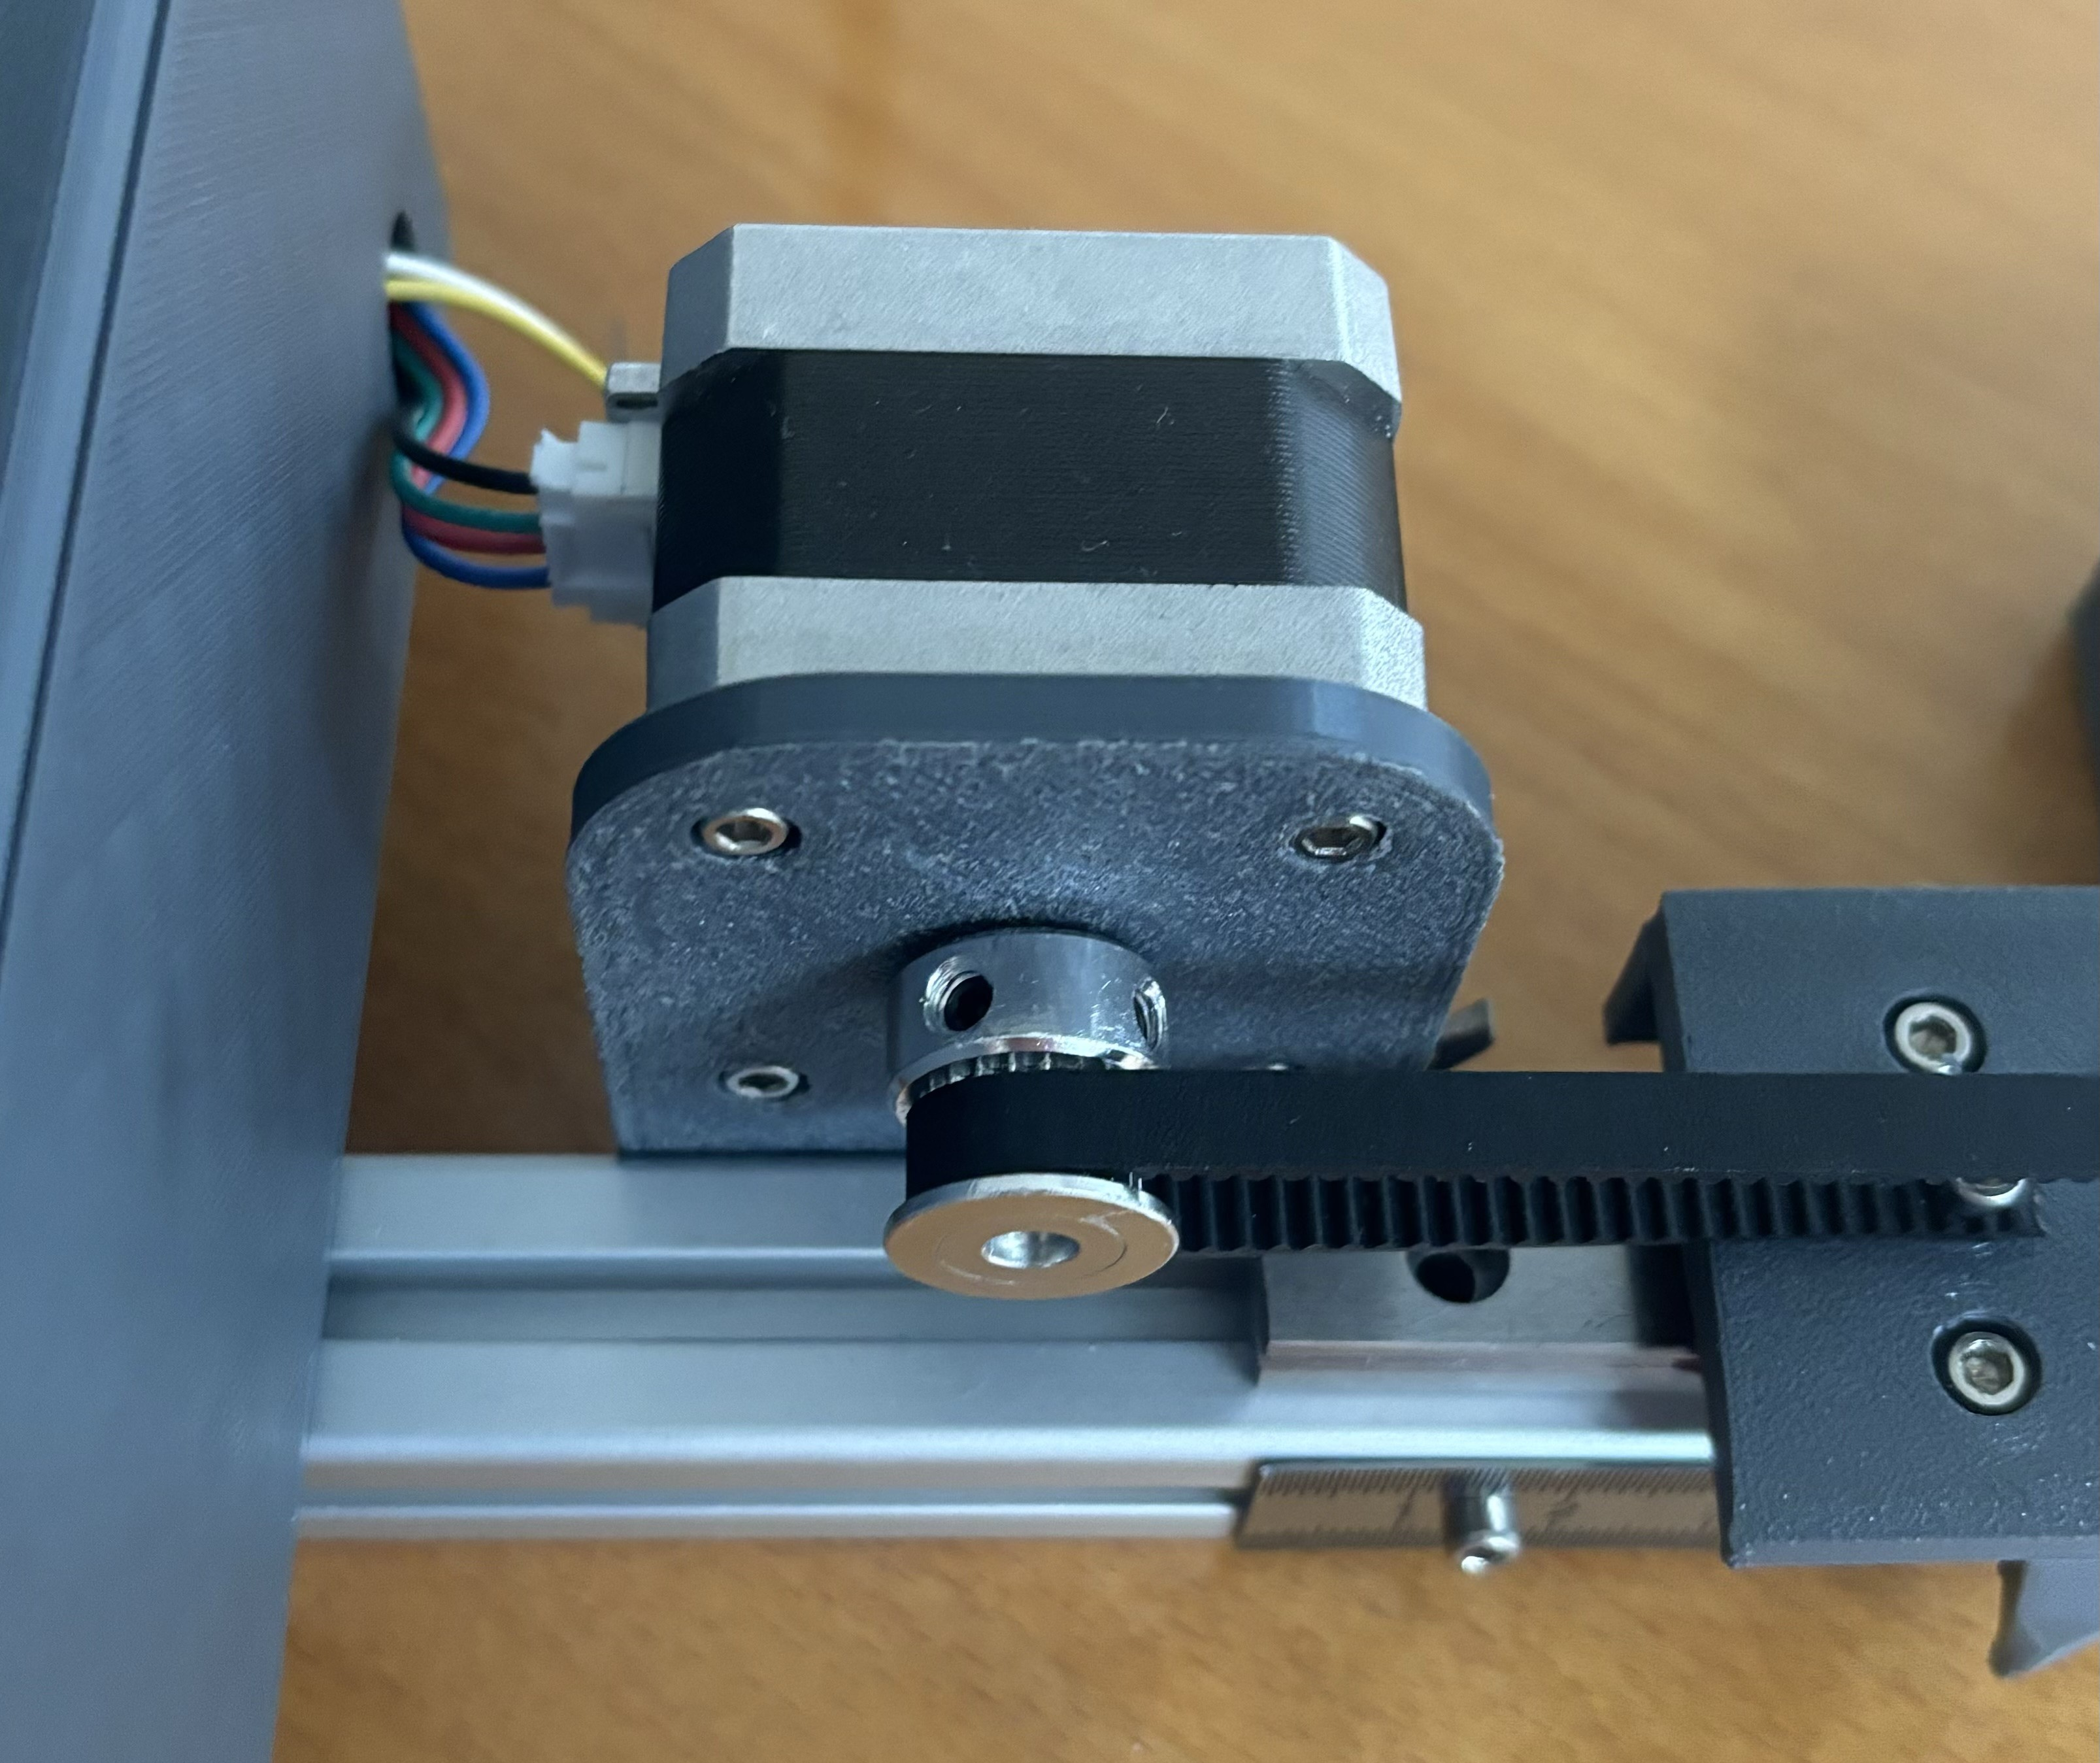
\includegraphics[width=\linewidth]{images/Schrittmotor}
			\end{tikzfigure}	
		}
		\block{Quellen}
		{
			\begin{itemize}
				\item R. Hagl. Elektrische Antriebstechnik. 3., überarbeitete und erweiterte Auflage. München: Hanser, 2021. isbn: 978-3-446-46572-5.
				\item G. Babiel. Elektrische Antriebe in der Fahrzeugtechnik: Lehrund Arbeitsbuch. 5. Auflage. Wiesbaden und Heidelberg: Springer Vieweg, 2023. isbn: 978-3-658-40585-4.
				\item Gemsmotor. Nema 17-Datasheet.
			\end{itemize}
		}
	}
	
	
	\column{0.6}
	{
		\colorlet{blocktitlebgcolor}{blue}
		\block{Herausforderungen}
		{
			Das Projekt lässt sich in drei verschiedene Teilprojekte unterteilen, die zum Abschluss der Aufgabe führen. Zuerst ist da die Konstruktion des Demonstrators und die hierfür benötigte Auswahl der Hardware-Teile. Vorgabe war, dass der Aufbau nicht zu komplex ist und man sich so auf die wesentlichen Teile konzentriert. Außerdem ist die Arbeit mit der Arduino IDE und die Programmierung des Arduino ein weiterer Teil. Als letzten Punkt ist der Umgang mit den elektronischen Bauteilen zu erwähnen. Der Umgang mit den elektronischen Bauteilen sollte unter großer Vorsicht geschehen, sodass diese nicht durch den elektrischen Strom beschädigt werden.
		}
		\block{Lösungsansatz}
		{
			Durch die Ausarbeitung der Herausforderungen, können Lösungsansätze	entwickelt werden. Vorab wurde eine erste Konzeptskizze angefertigt, aus der Ideen entstanden. Im ersten Konzept sollte der Schrittmotor eine Plattform über einen Riementrieb axial verfahren. Dabei sollte der Verfahrweg der Plattform über einen Abstandssensor mit einem vorher definierten Abstand zu einem Objekt, geregelt werden. Wird das Objekt näher oder weiter entfernt vom Abstandssensor bewegt, verfährt die Plattform mit einem definierten Abstand mit. Alle vorhandenen Bauteile sollten an einem Alu-Profil befestigt werden. Aufgrund der hohen Komplexität wurde die Plattform inklusive des Abstandssensors, aus dem zweiten Konzept entfernt. Stattdessen wird auf dem Schlitten der Linearführung, ein Zeiger und auf dem Alu-Profil, ein Lineal integriert. Mittels verschiedener Stufen soll der Schrittmotor unterschiedliche Geschwindigkeiten demonstrieren. Gegenüber dem zweiten Konzept wurde die Hardware aus Transportiergründen mit auf dem Aluprofil verlegt und erhielt zum Schutz ein Gehäuse.
		}
		\block{Zukünftige Projekte}
		{
			\begin{itemize}
				\item Aktive Geschwindigkeits- und Beschleunigungsregelung durch Beschleunigungssensor
				\item Manuelle Eingabe von Beschleunigung und Geschwindigkeit
				\item Manuelle Eingabe des Verfahrweges
			\end{itemize}
		}
	}
\end{columns}

\end{document}

